\section{Fähigkeiten}
\begin{frame}
\tableofcontents[currentsection]
\end{frame}
%\frame{\tableofcontents}
%\section{Einleitung}

\subsection{Einleitung}
\frame
{\frametitle{Fähigkeiten}
\begin{center}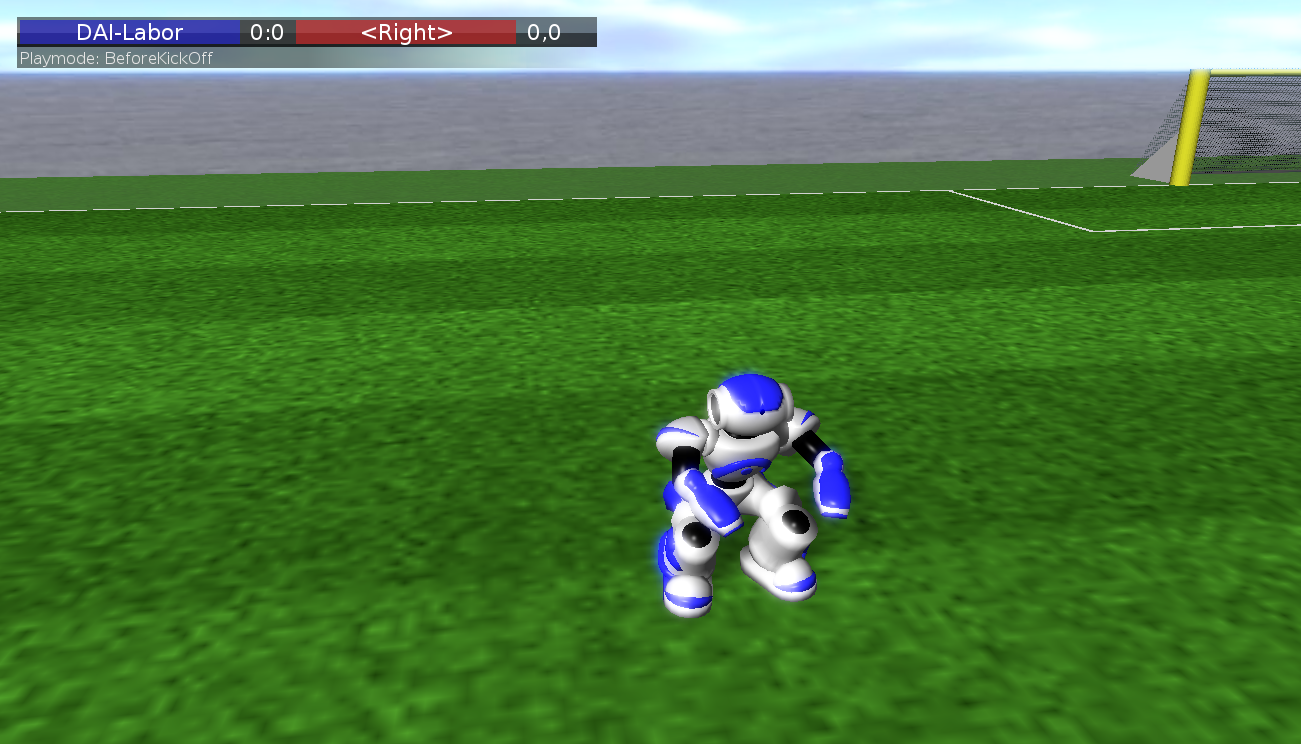
\includegraphics[height=6cm, center]{StandUpNAO}\end{center}
}
\frame
{
  \frametitle{Erste Überlegungen}
  \begin{itemize}
    \item zuerst wurde überlegt, was der fußballspielende NAO alles können muss
	\begin{itemize}
		\item Laufen und Drehen (Movement-Gruppe)
    		\item Schießen
    		\item Kopf bewegen
    		\item Arm bewegen
    		\item Dribbeln
    		\item Aufstehen
    	\end{itemize}
    \item spieziell für den Torwart
    \begin{itemize}
    		\item Parade
    		\item Aufstehen
    \end{itemize}
  \end{itemize}
}

\subsection{Umsetzung}
\frame{\frametitle{Keyframe und Keyframe-Engine}
\begin{itemize}
	\item Keyframe
	\begin{itemize}
		\item besteht aus Frames, die für die einzelnen Gelenke die Winkel angeben, die zu einem bestimmten Zeitpunkt erreicht werden sollen
	\end{itemize}
	\item Keyframe-Engine
	\begin{itemize}
		\item berechnet die Geschwindigkeiten der Gelenke für den nächsten Zyklus
	\end{itemize}
	\item der Kopf soll sich unabhängig von den restlichen Keyframe bewegen können
\end{itemize}
}

\frame{\frametitle{Berechnungsformeln}
für jedes Gelenk:\\
\begin{equation}
\varphi = \frac{20ms \cdot (Keyframe\varphi - (\varphi_{aktuell} + \varphi_{letzter Zyklus}))}{\Delta t_{Frame}- \Delta t_{vergangen}} \label{winkel}
\end{equation}
\begin{equation}
\omega = \frac{rad(\varphi)}{\underbrace{20 * 0,001}_{\text{20ms}}}
\end{equation}
Der berechnete Winkel (\ref{winkel}) wird für den nächsten Zyklus gespeichert und die Geschwindigkeiten and den Socket weitergeleitet.
}

\frame{\frametitle{Interfaces zu Taktikgruppe I}
\begin{itemize}
	\item Variable working: gibt an ob noch ein Keyframe gestartet ist, der nicht abgebrochen werden darf
	\item Funktion work: muss in jedem Zyklus aufgerufen werden; wenn aktuell eine Bewegung ausgeführt wird, wird diese fortgesetzt
\end{itemize}
}

\frame{\frametitle{Interfaces zu Taktikgruppe II}
Mit den folgenden Funktionsaufrufen werden die Keyframes gestartet:
\begin{itemize}
	\item stand() (Grundhaltung einnehmen)
	\item stand\_ up\_ from\_ back() (vom Rücken aufstehen)
	\item stand\_ up\_ from\_ front() (vom Bauch aufstehen)
	\item kick1() (erster Kick)
	\item lookAround() (umschauen)
\end{itemize}
}

\frame{\frametitle{Ausbau der Fähigkeiten}
Welche weiteren Fähigkeiten noch implementiert werden:
\begin{itemize}
	\item head\_ move(angle) (horizontale Kopfbewegung um bestimmten Winkel)
	\item head\_ stop() (lässt den Kopf anhalten)
	\item head\_ reset() (Kopf geradeaus sehen lassen)
	\item Torwart: Parade und evtl. spezielles Aufstehen
	\item Verbesserung des Kicks und weitere Schüsse
\end{itemize}
}